\documentclass[12pt, a4paper]{article}
\usepackage[utf8]{inputenc}
\usepackage[russian]{babel}
\usepackage[pdftex]{graphicx, color}
\usepackage{amsmath}
\usepackage{amsfonts}
\usepackage{amssymb}
\usepackage{amsthm}
\usepackage[left=2cm,right=1.5cm,top=1.5cm,bottom=2cm]{geometry}
\usepackage{indentfirst}
\usepackage{hyperref}

\usepackage{pbox}

\usepackage{setspace}
\onehalfspacing
\graphicspath{{pic/}}

\begin{document}

	\thispagestyle{empty}

	\begin{singlespace}
	\begin{titlepage}
		\begin{center}
			
\includegraphics[height = 3cm]{msu.png}

			{\scshape Московский государственный университет имени М.~В.~Ломоносова}\\
			Факультет вычислительной математики и кибернетики\\
			\centerline{\hfill\hrulefill\hrulefill\hrulefill\hrulefill\hfill}

			\vfill

			{\LARGE Отчет к пятому заданию практикума на ЭВМ: \\ Нейросетевой разреженный автокодировщик}

			\vspace{1cm}

		\end{center}

		\vfill
		\begin{flushright}
			\textit{Студент 3 курса ВМК (317 группа):}\\
				Оспанов А.М.

			\vspace{5mm}

		\end{flushright}

		\vfill

		\begin{center}
		Москва, 2015
		\end{center}
	\end{titlepage}
	\end{singlespace}

	\tableofcontents


	\newpage
	\section{Введение}
		Данный отчет написан к пятому заданию практикума на ЭВМ 317 группы. Тема задания: Нейросетевой разреженный автокодировщик. Отчет написан студентом 317 группы -- Оспановым Аятом.

		В данной работе был реализован нейросетевой разреженный автокодировщик. Были проведены исследования на качество классификации на исходных данных и на данных, полученных сокращением размерности

	\newpage
	\section{Основная часть}
		\subsection{Математические выкладки}
			Начнем с математических подготовок перед написанием кода. В документе задания были приведены частные производные в случае следующей функции потерь: $$J_0(W, b; x, y) = \frac{1}{2} ||h_{W,b}(x) - y || ^ 2$$

			А в случае с функцией потерь вида: $$J(W, b; x, y) = J_0(W, b; x, y) + \frac{\lambda}{2} \sum\limits_{l=1}^{n_{l-1}} \sum\limits_{i=1}^{s_l} \sum\limits_{j=1}^{s_{l+1}} (W_{ji} ^ {(l)}) ^ 2 + \beta \sum\limits_{j=1}^h KL(\rho || \hat{\rho_j})$$
			мы имеем изменения некоторых формул и получаем следующие формулы для алгоритма обратного распространения ошибки:
			$$\delta_i^{(l)} = \bigg(
									\sum\limits_{j=1}^{s_{l+1}} W_{ji}^{(l)}\delta_j^{(l+1)} +
									\beta \Big(-\frac{\rho}{\hat{\rho_j}} + \frac{1 - \rho}{1 - \hat{\rho_j}}\Big)
							   \bigg)f'(z_i^{(l)}) \quad (1)$$ 
			$$\frac{\partial }{\partial W_{ij}^{(l)}} J(W, b; x, y) = a_j^{(l)} \delta_i^{(l+1)} + \lambda W_{ij}^{(l)} \quad (2)$$\

			Теперь выведем эти формулы:

			Вторая формула очевидна: первое слагаемое приведено в Ликбезе, а второе слагаемое вычисляется взятием прозводной квадратной функции.

			Выведем первую формулу: первое слагаемое приведено в Ликбезе. Второе слагаемое находится взятием производной дивергенции Кульбака — Лейблера:

			$$\frac{\partial}{\partial z_i^{(l)}} KL(\rho || \hat{\rho_i}^{(l)}) = \frac{\partial KL}{\partial \rho_i^{(l)}} \frac{\partial \rho_i^{(l)}}{\partial z_i^{(l)}} = \Big(-\frac{\rho}{\rho_i^{(l)}} + \frac{1 - \rho}{1 - \rho_i^{(l)}}\Big) \sigma '(z_i^{(l)})$$

			Учитывая, что слагаемое с дивергенцией Кульбака — Лейблера имеет коэфициент $\beta$, получим окончательно формулу (1).

		\newpage
		\subsection{Сравнение градиентов}
			\begin{center}{\bfСравнение градиентов функции autoencoder\_loss и функции compute\_gradient}\end{center}

			Проверка делалась на маленькой выборке (подвыборке нормализованных патчей), иначе функция compute\_gradient вызывалась бы столько раз, сколько размер переменной, по которой высчитывается градиент. В этом и есть большой плюс алгоритма обратного распространения ошибки (он высчитывает градиент всего за один вызов)

			В итоге, точность совпадения градиентов получилась $10^{-7}$, что доказывает правильность математических выкладок и написания этого алгоритма.
		
		\newpage
		\subsection{Зависимость визуализиаций от гиперпараметров} \label{sssec:p3}
			% \begin{center}{\bfЗависимость визуализиаций от гиперпараметров}\end{center}

			В ходе исследований зависимости картинки на скрытом слое, получились следующие результаты (максимальное количество итераций 10000; Стандартные значения: $\lambda = 0.0001$ $\beta = 3$ $\rho = 0.01$; Если не указан параметр в таблице, то считается, что он стандартный):
			\begin{center}
			{\bfПлохие параметры \\}

			\begin{tabular}{l l l}
				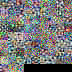
\includegraphics[width=5cm]{hidden_10000it_l=0_b=0.png} &
				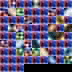
\includegraphics[width=5cm]{hidden_10000it_6354it_b=0-03.png} &
				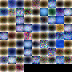
\includegraphics[width=5cm]{hidden_10000it_333it_l=0-01_b=1.png} \\

				\pbox{5cm}{Итераций: 10000\\ $\lambda = 0$ $\beta = 0$ \\} &
				\pbox{5cm}{Итераций: 6354\\ $\beta = 0.03$ \\} &
				\pbox{5cm}{Итераций: 333\\ $\lambda = 0.01$ $\beta = 1$ \\} \\
				

				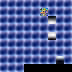
\includegraphics[width=5cm]{hidden_10000it_816it_l=0-001_b=2.png} &
				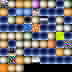
\includegraphics[width=5cm]{hidden_10000it_698it_spars=0-001.png} &
				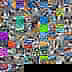
\includegraphics[width=5cm]{hidden_10000it_698it_spars=0-1.png} \\

				\pbox{5cm}{Итераций: 816\\ $\lambda = 0.001$ $\beta = 2$ \\} &
				\pbox{5cm}{Итераций: 698\\ $\rho = 0.001$ \\} &
				\pbox{5cm}{Итераций: 698\\ $\rho = 0.1$ \\} \\
			\end{tabular}

			{\bfХорошие параметры \\}

			\begin{tabular}{l l l}
				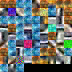
\includegraphics[width=5cm]{hidden_10000it_7399it_std.png} &
				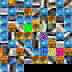
\includegraphics[width=5cm]{hidden_10000it_9151it_std.png} &
				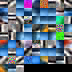
\includegraphics[width=5cm]{hidden_10000it_b=0-3.png} \\

				\pbox{5cm}{Итераций: 7399} &
				\pbox{5cm}{Итераций: 9151} &
				\pbox{5cm}{Итераций: 10000\\ $\beta = 0.3$} \\

			\end{tabular}
			\end{center}

			Из таблицы видно, что при уменьшении $\rho$ или $\lambda$, картинки ухудшаются. А вот $\beta$ влияет на шум в этих картинках. Чем меньше $\beta$, тем меньше шума. Таким образом, $\rho = 0.01$, $\lambda = 0.0001$ и $\beta = 0.3$ являются оптимальными параметрами.

		\newpage
		\subsection{Сравнение точности классификации} \label{sssec:p4}
			% \begin{center}{\bfСравнение точности классификации}\end{center}

			Для классификации был выбран метод RandomForest, так как этот классификатор дает самую большую точность из всех перепробованных (SVM-Linear, SVM-RBF, kNN, DesTree) и работает быстро. А также был использован Байесовский классификатор для сравнения результатов.

			Сначала протестируем классификатор по значению интенсивности каналов изображений. Обучим на выборке train, протестируем на выборке test. Точность классификатора для исходных данных на Random Forest получилась 0.333375, на наивном байесе 0.323875

			Далее будем сравнивать сеть с одним скрытым слоем и тремя скрытыми слоями.

			\begin{center}{\bfСеть с одним скрытым слоем}\end{center}

			Для классификации, из выборки train берутся всевозможные патчи с некоторым шагом и соответствующие патчи из test. Результат можно увидеть в следующей таблице:

			\begin{center}
			\begin{tabular}{l l l}
				Размер шага & Random Forest & Наивный байес \\
				4 & 0.342375 & 0.424375\\
				6 & 0.328000 & 0.41775\\
				10 & 0.324250 & 0.39525\\
			\end{tabular}
			\end{center}

			Из этой таблицы можно сделать вывод о том, что чем меньше шаг, т.е. чем больше признаков, тем больше точность. А прирост точности по сравнению с исходными данными не очень большой, порядка 2-3\%, но количество признаков снизилось, следовательно скорость классификации возрасла

			\begin{center}{\bfСеть с тремя скрытыми слоями}\end{center}

			Для классификации, делаются те же манипуляции с патчами, но в этот раз используется трехслойная сеть. Результат можно увидеть в следующей таблице:

			\begin{center}
			\begin{tabular}{l l l}
				Размер шага & Random Forest & Наивный байес \\
				4 & 0.293625 & 0.328625\\
				6 & 0.286625 & 0.319875\\
				10 & 0.274375 & 0.309375\\
			\end{tabular}
			\end{center}

			Как и в однослойной сети, при росте шага, уменьшается точность. Но прироста в точности по сравнению с исходными данными, и тем более с однослойной сетью - нет. Но есть прирост в скорости по сравнению с однослойной сетью, но в ущерб точности.


		\newpage
		\subsection{Бонус 1}
			Исследуем зависимость точности классификации от количества патчей. В следующей таблице визуализированы веса на скрытых слоях для разного количества патчей:

			\begin{center}
			\begin{tabular}{l l l}
				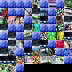
\includegraphics[width=5cm]{hidden_100.png} &
				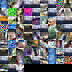
\includegraphics[width=5cm]{hidden_500.png} &
				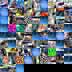
\includegraphics[width=5cm]{hidden_1000.png} \\

				\pbox{5cm}{100 патчей} &
				\pbox{5cm}{500 патчей} &
				\pbox{5cm}{1000 патчей} \\

				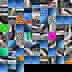
\includegraphics[width=5cm]{hidden_3000.png} &
				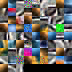
\includegraphics[width=5cm]{hidden_6000.png} &
				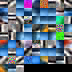
\includegraphics[width=5cm]{hidden_10000it_b=0-3.png} \\

				\pbox{5cm}{3000 патчей} &
				\pbox{5cm}{6000 патчей} &
				\pbox{5cm}{10000 патчей} \\
			\end{tabular}
			\end{center}

			Из картинок видно, что качество улучшается с увеличением количества патчей

			А в следующей таблице и диаграмме представлены точности в зависимости от количества патчей:

			\begin{center}
			\begin{tabular}{| l | l | l | l | l | l | l |}
				\hline
				Количество патчей & 100 & 500 & 1000 & 3000 & 6000 & 10000 \\
				\hline
				Точность & 0.326125 & 0.327375 & 0.325625 & 0.326125 & 0.337375 & 0.345875 \\
				\hline
			\end{tabular}
			\end{center}

			\begin{center}
				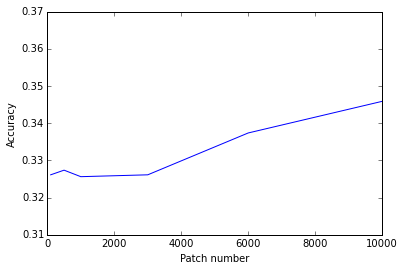
\includegraphics[width=8cm]{accuracyFromPatchSize.png}
			\end{center}

			Из графика видно, что зависимость точности от количества патчей является линейной в приближении

	\newpage
	\section{Заключение}
		В ходе исследований были подобраны оптимальные гиперпараметры для дальнейших исследований (см. \textit{~\nameref{sssec:p3}}). Далее были исследованы точности классификации для основных данных (интенсивности каналов), данных, полученных из однослойного автокодировщика и трехслойного автокодировщика (см. \textit{~\nameref{sssec:p4}}). В результате этих исследований выяснилось, что данные из однослойной сети лучше классифицируются нежели данные из трехслойной сети. Также было замечено, что в случае Байесовского классификатора точность на данных из однослойной сети возрастает на порядок (примерно 10\%).

		При классификации с помощью слуйчаного леса точность на данных из сети меняется на 1-2\% по сравнению с исходными данными, а в случае Байесовского классификатора прирост около 10\%. Это можно объяснить тем, что для метода Random Forest нужно много данных для более точной классификации, следовательно прирост маленький, т.к. мы уменьшаем признаковое пространство. Но прирост все таки есть. Объясняется это тем, что мы ``выделили'' основные (базисные) признаки. А в случае наивного байеса данные должны быть как можно более информативными, т.е. мы должны выделить более важные признаки. А это то, что делает автокодировщик (``выделяет базис''). Это же можно заметить и в случае линейного классификатора.

\end{document}
